\section{Kịch bản giao tiếp của chương trình}
\subsection{Giao thức trao đổi giữa client và server}
Server và client trao đổi với nhau thông qua giao thức UDP.
\subsection{Cấu trúc của thông điệp}

\large\textbf{Một thông điệp có tổng cộng \texttt{1024 bytes}.} 
\begin{enumerate}
\item \textbf{Đối với thông điệp từ server có 2 loại sau đây}
\normalsize
\begin{enumerate}
\item \textit{Thông điệp gửi số lượng thông điệp cần nhận cho data:} \texttt{|padding|len|}

Có dạng \texttt{<1021 bytes 0>xyz} (\texttt{xyz} là ba chữ số).

Gồm 2 trường theo thứ tự đó với các mô tả chi tiết sau đây:

\begin{enumerate}
\item \texttt{padding}: Gồm các null bytes (các bytes \texttt{\textbackslash x00}) chèn vào trước trường \texttt{len} sao cho tổng thông điệp có đủ 1024 bytes.

\item \texttt{len}: kiểu \texttt{str}, thể hiện số lượng thông điệp (tối đa 3 bytes).
\end{enumerate}

\item \textit{Thông điệp gửi từng phân data:} \texttt{|ID|data|hash|}

Có dạng \texttt{xyz<data: 981><hash: 40>} (\texttt{xyz} là ba chữ số).

Gồm 3 trường theo thứ tự đó với các mô tả chi tiết sau đây:

\begin{enumerate}
\item \texttt{ID}: Kiểu \texttt{str} gồm 3 ký tự thể hiện số trong đoạn \texttt{[000; 999]} (3 bytes).

\item \texttt{data}: Kiểu \texttt{byte}, gồm 981 (1024 - 43) ký tự (981 bytes).

\item \texttt{hash}: Kiểu \texttt{str}, gồm 40 ký tự (40 bytes) được tạo khi hash data bằng \texttt{thuật toán SHA1} để kiểm lỗi. \textit{40 bytes này mô tả một số nguyên 20 bytes = 160 bits trong hệ thập lục phân.}
\end{enumerate}


\end{enumerate}
\large
\item \textbf{Đối với thông điệp từ client có 6 loại sau đây.}
\normalsize

\begin{enumerate}
\item \textit{Thông điệp xác nhận số lượng:} \texttt{|specifier|len|padding|}

Có dạng \texttt{ACK{\_}LEN{\_}xyz<1013 bytes 0>} (\texttt{xyz} là ba chữ số).

Gồm 3 trường theo thứ tự đó với các mô tả chi tiết sau đây:

\begin{enumerate}
\item \texttt{specifier}: kiểu \texttt{str}, là chuỗi ký tự \texttt{"ACK\_{LEN}\_"} (8 bytes)
\item \texttt{len}: kiểu \texttt{str}, là số lượng thông điệp đã nhận từ server, gồm 3 ký tự thể hiện số trong đoạn \texttt{[000; 999]} (3 bytes)
\item \texttt{padding}: gồm 1013 (1024 - 8 - 3) bytes \texttt{\textbackslash x00}.
\end{enumerate}

\item \textit{Thông điệp xác nhận phần data:} \texttt{|specifier|id|padding|}

Có dạng \texttt{ACK{\_}xyz<1017 bytes 0>} (\texttt{xyz} là ba chữ số).

Gồm 3 trường theo thứ tự đó với các mô tả chi tiết sau đây:

\begin{enumerate}
\item \texttt{specifier}: kiểu \texttt{str}, là chuỗi ký tự \texttt{"ACK{\_}"} (4 bytes)
\item \texttt{id}: kiểu \texttt{str}, là thứ tự của thông điệp nhận từ server, gồm 3 ký tự thể hiện số trong đoạn [000; 999] (3 bytes)
\item \texttt{padding}: gồm 1017 (1024 - 4 - 3) bytes \texttt{\textbackslash x00}.
\end{enumerate}

\item \textit{Thông điệp yêu cầu thông tin toàn bộ địa điểm:} \texttt{|command|padding|}

Có dạng \texttt{GIV{\_}ALL<1017 bytes 0>}

Gồm 2 trường theo thứ tự đó với các mô tả chi tiết sau đây:

\begin{enumerate}
\item \texttt{command}: kiểu \texttt{str}, là chuỗi ký tự \texttt{"GIV{\_}ALL"} (7 bytes)
\item \texttt{padding}: gồm 1017 (1024 - 7) bytes \texttt{\textbackslash x00}.

\end{enumerate}

\item \textit{Thông điệp yêu cầu thông tin chi tiết 1 địa điểm:} \texttt{|command|id|padding|}

Có dạng \texttt{GIV{\_}DETAIL{\_}<id: x bytes><1013 - x bytes 0>} 

Gồm 3 trường theo thứ tự đó với các mô tả chi tiết sau đây:

\begin{enumerate}
\item \texttt{command}: kiểu \texttt{str}, là chuỗi ký tự \texttt{"GIV{\_}DETAIL{\_}"} (11 bytes)
\item \texttt{id}: kiểu \texttt{str}, thể hiện id của địa điểm cần lấy.
\item \texttt{padding}: Gồm các bytes \texttt{\textbackslash x00} điền cho đủ 1024 bytes.
\end{enumerate}

\item \textit{Thông điệp yêu cầu ảnh đại diện 1 địa điểm:} \texttt{|command|id|padding |}

Có dạng \texttt{GIV{\_}AVT{\_}<id: x bytes><1016 - x bytes 0>} 

Gồm 3 trường theo thứ tự đó với các mô tả chi tiết sau đây:

\begin{enumerate}
\item \texttt{command}: kiểu \texttt{str}, là chuỗi ký tự \texttt{"GIV{\_}AVT{\_}"} (8 bytes)
\item \texttt{id}: kiểu \texttt{str}, thể hiện id của địa điểm cần lấy.
\item \texttt{padding}: Gồm các bytes \texttt{\textbackslash x00} điền cho đủ 1024 bytes.
\end{enumerate}

\item \textit{Thông điệp yêu cầu ảnh tại 1 địa điểm:} \texttt{|command|position|separator|id|padding|}

Có dạng \texttt{GIV{\_}IMG{\_}xyz{\_}<id: t bytes><1012 - t bytes 0>} (\texttt{xyz} là ba chữ số).

Gồm 5 trường theo thứ tự đó với các mô tả chi tiết sau đây:

\begin{enumerate}
\item \texttt{command}: kiểu \texttt{str}, là chuỗi ký tự \texttt{"GIV{\_}IMG{\_}"} (8 bytes)
\item \texttt{position}: kiểu \texttt{str}, là thứ tự trong danh sách ảnh cần lấy, gồm 3 ký tự thể hiện số trong đoạn \texttt{[000; 999]} (3 bytes)
\item \texttt{separator}: kiểu char, là ký tự '{\_}'
\item \texttt{id}: kiểu \texttt{str}, thể hiện id của địa điểm cần lấy.
\item \texttt{padding}: Gồm các bytes \texttt{\textbackslash x00} điền cho đủ 1024 bytes.
\end{enumerate}
\end{enumerate}
\end{enumerate}
\subsection{Cách tổ chức cơ sở dữ liệu}
Dữ liệu được lưu trong tập tin \texttt{db.json} thành các bộ với các trường thông tin sau:
\begin{itemize}
\item \texttt{id}: gồm ba ký tự kiểu \texttt{char}, là viết tắt tên địa điểm.
\item \texttt{name}: tên đầy đủ của địa điểm tương ứng.
\item \texttt{coordinate}: tọa độ vị trí trung tâm của địa điểm theo thứ tự vĩ độ và kinh độ. Địa điểm có vĩ độ dương nằm ở phía Bắc đường xích đạo, vĩ độ âm nằm ở phía Nam đường xích đạo. Địa điểm có kinh độ dương nằm ở phía Đông kinh tuyến gốc, kinh độ âm nằm ở phía Tây kinh tuyến gốc.
\item \texttt{description}: đoạn mô tả ngắn về địa điểm tương ứng.
\item \texttt{avatar}: lưu đường dẫn tương đối (so với tập tin \texttt{db.json}) đến ảnh đại diện của địa điểm.
\item \texttt{images}: lưu danh sách đường dẫn tương đối (so với tập tin \texttt{db.json}) đến các hình ảnh của địa điểm.
\end{itemize}
Thư mục \texttt{images} được chia thành các thư mục con, mỗi thư mục con có tên là các \texttt{id}, trong thư mục tương ứng bao gồm một hình đại diện \texttt{avt.jpg}, và các hình ảnh minh họa khác \texttt{img*.jpg}, trong đó * là số thứ tự của hình ảnh tương ứng.
Các thông tin được đưa vào cơ sở dữ liệu dưới dạng mã Unicode.
\begin{figure}[H]
\center{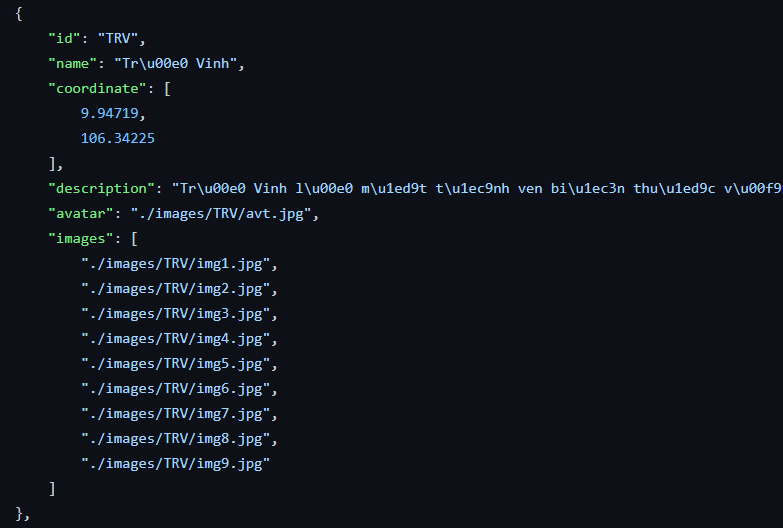
\includegraphics[scale=0.75]{protocol/db_example}}
\caption{Ví dụ về cấu trúc lưu trữ dữ liệu}
\end{figure}

\begin{figure}[H]
\center{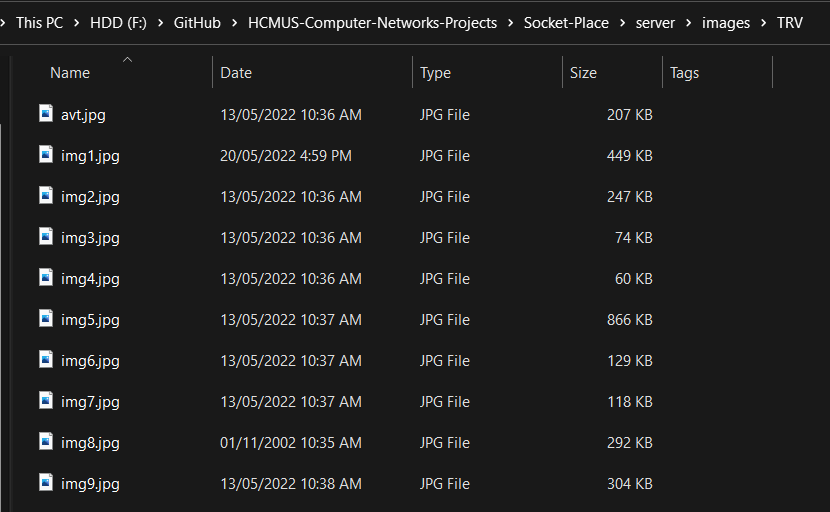
\includegraphics[scale=0.75]{protocol/img_example}}
\caption{Ví dụ về cấu trúc thư mục con của \texttt{images}}
\end{figure}

\subsection{Quá trình truyền từ client lên server}
\begin{enumerate}
\item Đoạn dữ liệu ban đầu sẽ được xử lý thành danh sách các thông điệp kích thước 1024.
\item Server gửi số lượng thông điệp cho client và chờ \texttt{ACK}.
\item Sử dụng thuật toán \texttt{Sliding window} với kích thước 5 để truyền:
\begin{itemize}
\item Phía server
\begin{breakablealgorithm}
  \caption{Phía server}
  \begin{algorithmic}[1]
    \Function{SWServer}{} 
	\State $tds \gets $ danh sách thông điệp cần truyền
	\State $l\_tds \gets $ độ dài danh sách
    \State $size \gets $ kích thước cửa sổ = $5$
    \State $i \gets 0 $
    \While{$ i < l\_tds$}
    	\State $struyen \gets $ số lượng truyền = $\min\left( {size,{\text{ }}l\_tds{\text{ }} - {\text{ }}i} \right)$
    	\State $kt \gets$ mảng đánh dấu kích thước struyen
    	\While{$kt$ chưa được đánh dấu hết}
    		\State truyền lần lượt toàn bộ cửa sổ hiện tại ($i \to i + struyen$)
    		\State thực hiện nhận ACK $struyen$ lần, đánh dấu $ID$ vào $kt$
    		\State nếu quá giờ nhận ACK, coi như gói bị mất và truyền lại
    	\EndWhile
    	\State $i \gets i + size$ (dịch tới cửa sổ tiếp theo)
    \EndWhile
    \EndFunction
  \end{algorithmic}
\end{breakablealgorithm}

\end{itemize}
\end{enumerate}